% !TEX root = ../thesis.tex

In this chapter, we look at ways to implement the loopy belief propagation (LBP) algorithm on an arbitrary MRF with continuous state-spaces. We concentrate in particular on the representation of the messages and the computation of message updates in the LBP algorithm. 

In this chapter, we consider the \emph{nonparametric belief propagation} (NBP) algorithm of \citet{sudderth03} and the \emph{particle belief propagation} algorithm of \citet{ihler09}. We then discuss our \emph{expectation particle belief propagation} (EPBP) algorithm \citep{lienart15} and discuss how it can improve upon both. \check{jul19}

% !!!!!!!!!!!!!!!!!!!!!!!!!!!!!!!!!!!!!!!!!!!!!!!!!!!!!!!!!!!!!!!!!!!!!!!!!!!!!!!!!!!!!!!!!!!!!!!!!!
\section{\label{sec:LBPonCS}Loopy Belief Propagation on Continuous State-Spaces}
At point \ref{point:LBP}, we had shown that, at iteration $n$ of the LBP algorithm, the messages are obtained by computing the following integral:
\eqa{
	m^{n}_{ts}(x_{s}) &=& \int \psi_{st}(x_{s},x_{t})M^{n}_{t s}(x_{t})\dx_{t}\label{eq:mess-update-2}
}
where the pre-messages are given by 
\eqa{
	M_{st}^{n}(x_{s}) &=& \psi_{s}(x_{s}) \prod_{r\in\partial s\backslash t} m^{n-1}_{rs}(x_{s}).
}
Ultimately, we are interested in computing the beliefs obtained by multiplying message and pre-message: $B_{s}^{n}(x_{s}) = m^{n}_{ts}(x_{s})M^{n}_{st}(x_{s})$. There are a few main computational problems to tackle when attempting to run this algorithm in a continuous state space. First, the messages need to be represented in a tractable fashion. Second, the message updates need to be computable and the results easily expressible in the chosen representation system. Lastly, we need to be able to easily compute expected values with respect to the resulting estimators for the beliefs. We discuss below two existing methods attempting to tackle those issues.
%%%%%%%%%%%%%%%%%%%%%%%
\subsection{Nonparametric Belief Propagation}

In \citet{sudderth03}, the authors suggest representing the messages in the LBP iterations as mixtures of Gaussians:
\eqa{	
	\widehat m^{\text{NBP}}_{ts}(x_{s}) &:=& \sum_{i=1}^{M} w_{s}^{i}\,\mathcal N(x_{s};\mu^{i}_{s},\Lambda_{s}). \label{eq:nbp-representation}
}
They call their algorithm \emph{nonparametric belief propagation} (NBP). In order to make computations more efficient, the authors restrict the covariance matrices to be diagonal.
As indicated in the paper, the representation \eqref{eq:nbp-representation} makes sense only when the messages are finitely integrable. To guarantee this, the authors require that all potentials satisfy the following constraints:
\eqa{	
	\sup_{x_{t}} \int \psi_{st}(x_{s},x_{t})\dx_{t} &<&\infty, \quad \text{and}\quad \int \psi_{s}(x_{s})\dx_{s} \esp<\esp \infty,\label{conditions NBP}
}
where the integrals are taken over the range of admissible values for the relevant variable. Provided these assumptions hold, the message updates are well defined and can be explicitly (and efficiently) computed. Computing the beliefs however, requires considering the product of mixtures of $M$ terms leading to a complex representation and an explosion in computational cost. In order to alleviate this, the authors suggest an importance sampling approach targeting the beliefs and fitting mixtures of Gaussians to the resulting weighted particles. 
The computation of the message updates \eqref{eq:mess-update-2} is thereby always done over a constant number of terms.\check{jul19}

\subsubsection*{Main issues}

A key weakness of the NBP algorithm is that the conditions \eqref{conditions NBP} do not hold in a number of important cases (the authors aknowledge this in a footnote of their paper). 
First, the node potentials $\psi_{u}$ are usually proportional to likelihoods of the form $p(y_{u}\st x_{u})$ which need not be integrable in $x_{u}$. In fact, for most non-Gaussian potentials, this is the case. Then, there exist applications for which the first integrability condition on edge potentials does not hold. In imaging applications for example, the edge potential can encode a measure of similarity between pixels which need not verify the first integrability condition as in \citet{nikolova00}. Finally, by definition of NBP as an approximated representation with a fixed number of Gaussians, it does not lead to consistent estimators of the LBP messages.\check{jul24, jul21, jul19}



%%%%%%%%%%%%%%%%%%%%
\subsection{\label{point:PBP}Particle Belief Propagation}

In \citet{ihler09}, the authors suggest a way to overcome the shortcomings of NBP by considering importance sampling to tackle the update of the LBP messages instead of working with mixtures of Gaussians. For a chosen proposal distribution $q_{u}$ on node $u$ and a draw of $N$ particles $X_{u}^{(i)}\simiid q_{u}$, the messages are represented via an importance sampling estimator of the corresponding integral:
\eqa{		
	&\widehat m_{st}^{\text{PBP}}(x_{t}) 
		:= \sum_{i=1}^{N}w^{(i)}_{st}\psi_{st}(X^{(i)}_{s},x_{t}), \quad\text{where}&	\label{eq:rep-PBP}\\[.4cm]
	&w^{(i)}_{st} 
		\esp\!\propto\esp\! \displaystyle{\widehat M^{\text{PBP}}_{st}(X_{s}^{(i)})\over q_{s}(X_{s}^{(i)})}, \quad\text{and}\quad
	\widehat M^{\text{PBP}}_{st}(x_{s}) \esp\!=\esp\! \psi_{s}(x_{s}) \prod_{r\in\partial s\backslash t} \widehat m^{\text{PBP}}_{rs}(x_{s}).&\nn
}

They call their algorithm \emph{particle belief propagation} (PBP).
This algorithm has the advantage that it does not explicitly require the integrability conditions \eqref{conditions NBP} to hold. 
In terms of choosing proposals, the authors suggest two potential choices: sampling from the local potential $\psi_{s}$, or sampling from the current belief estimate on the node. 
%For the latter, the authors suggest running a short MCMC simulation. \add{explain how they build representation of beliefs}

\subsubsection{Main issue}

The weak point of the PBP algorithm is the choice of proposal distributions.  A poor choice will lead to poor estimators of the messages which, over a few iterations of the LBP algorithm, can lead to poor representations of the beliefs.

The first suggestion by the authors to sample from the local potential is only valid if $\psi_{s}$ is integrable which, as we have mentioned earlier, is not the case in general. The second suggestion implies sampling from a distribution of the form
%
\eqa{		
	\widehat B_{s}^{\text{PBP}}(x_{s}) 
		&\propto& \psi_{s}(x_{s}) \prod_{r\in\partial s} \widehat m^{\text{PBP}}_{rs}(x_{s})	\label{eq:PBP proposal}
}
%
which is a product of mixtures of $N$ components. As in nonparametric BP, naive sampling of the proposal has complexity $\mathcal O {(N^{|\partial {s}|})}$ and is thus, in general, too expensive to consider.

Alternatively the authors suggest running a short MCMC simulation targeting it which reduces the complexity to order $\mathcal O {(|\partial {s}|N^{2})}$. Indeed, each MCMC iteration requires evaluating $\widehat B_{s}^{\text{PBP}}$ point-wise which has complexity $\mathcal O {(|\partial{s}|N)}$, and we need at least $\mathcal{O}(N)$ iterations of the MCMC simulation to produce the samples. Note that it is unclear how many more iterations are necessary to get $N$ \emph{good} samples. Running a short MCMC chain (to reduce computational cost) will therefore almost certainly lead to biased samples. In the code the authors shared with us, they run $N$ parallel random walk Metropolis-Hastings chains \citep[chapter 6]{robert04} for a fixed number of steps. This choice may have been motivated by a desire to control the complexity of the algorithm more accurately but it is at the expense of the quality of the samples obtained.

%%%%%%%%%%%%%%%%%%%%%%%%
\section{\label{sec:EPBP}Expectation Particle Belief Propagation}
As for the PBP algorithm, we consider importance sampling to build particle representations of the messages. In our method, however, we consider a \emph{sequence} of proposal distributions at each node from which one can cheaply sample particles at a given iteration of the LBP algorithm \citep{lienart15}.

The novelty of the approach is to propose a principled and automated way of designing a sequence of proposals in a tractable exponential family using the expectation propagation (EP) algorithm. The resulting method, which we call \emph{Expectation Particle Belief Propagation} (EPBP), does not suffer from the restrictive integrability conditions of the NBP algorithm and sampling is done exactly unlike the PBP algorithm which implies that we obtain consistent estimators of the LBP messages.

Further, the development of our method also formally shows that considering proposals close to the beliefs, as suggested by \cite{ihler09}, is a good idea.  Our core observation is that since sampling from a proposal of the form \eqref{eq:PBP proposal} using MCMC simulation is very expensive, we should consider using a more tractable proposal distribution instead. However it is important that the proposal distribution is constructed adaptively, taking into account evidence collected through the message passing itself. We propose to achieve this by using proposal distributions lying in a tractable exponential family, and adapted using EP.

%%%%%%%%%%%%%%%%
\subsection{Proposal selection for PBP}
In this point we discuss the ideal choice of proposal distributions when considering the PBP algorithm. We consider two connected nodes $s$ and $t$ at a a given iteration and assume we have already constructed particle based representations of all incoming messages into both $s$ and $t$ apart from the messages from $s$ to $t$ and from $t$ to $s$. 
We therefore have both pre-messages $\widehat M_{st}$ and $\widehat M_{ts}$ of the form:
%
\eqa{
	\widehat M_{st}(x_{s}) &\propto& \psi_{s}(x_{s}) \prod_{r\in \partial s \backslash t} \widehat m_{rs}(x_{s}).
}
%
This is illustrated in figure \ref{representation-edge-pbp}. 

\begin{figure}[!h]
\center
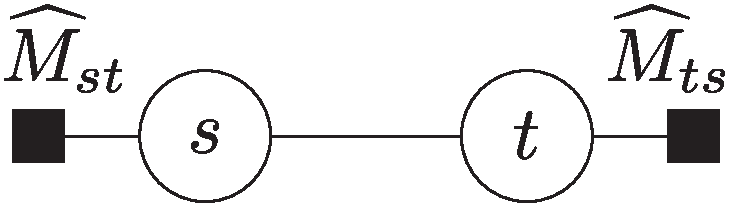
\includegraphics[width=.4\textwidth]{figures/general/belief-st}
\caption{\label{representation-edge-pbp}Illustration of the situation for an edge $(s,t)$: all messages coming into $s$ and $t$ have been approximated apart from the messages between $s$ and $t$. Therefore approximated pre-messages (denoted $\widehat M$) are available on both nodes. We are considering the problem of determining the best proposals on $s$ and $t$ in order to approximate the messages between $s$ and $t$ given the situation.}
\end{figure}

We would like to define $q_{s}$ and $q_{t}$ in a joint manner in such a way that all objects remain consistent with the LBP iterations. For that reason, we consider the joint belief $ B_{st}$ on $s$ and $t$ given the approximation to the pre-messages:
%
\eqa{	
	 B_{st}(x_{s},x_{t}) &\propto& \widehat M_{st}(x_{s}) \psi_{st}(x_{s},x_{t})\widehat M_{ts}(x_{t}).
}
%
The marginals of the joint belief are of the form
%
\eqa{
	B_{st}(x_{s}) &\propto& \widehat M_{ts}(x_{s}) \int \psi_{st}(x_{s},x_{t}) \widehat M_{ts}(x_{t})\dx_{t}\nn\\
	&\propto & \widehat M_{st}(x_{s}) m_{ts}(x_{s}),
}
%
where $m_{ts}$ is the exact (but intractable) LBP message given the pre-message approximation $\widehat M_{ts}$.
Following our point about defining $q_{s}$ and $q_{t}$ in a joint manner, let us consider $q_{s}q_{t}$ as a proposal for the joint belief $ B_{st}$.
We can then define an empirical distribution for it:
%
\eqa{
	\widehat{B}_{st}(x_{s},x_{t}) &\propto& \sum_{i,j=1}^{N} {\widehat M_{st}(X_{s}^{(i)})\psi_{st}(X_{s}^{(i)},X_{t}^{(j)})\widehat M_{ts}(X_{t}^{(j)}) \over q_{s}(X_{s}^{(i)})q_{t}(X_{t}^{(j)})} \delta_{(X_{s}^{(i)},X_{t}^{(j)})}(x_{s},x_{t}). \label{eq:pbp-particle-joint-belief}
}
%
Marginalising this approximation over $x_{t}$ leads to
%
\eqa{
	\widehat{B}_{st}(x_{s}) &\propto& \sum_{i=1}^{N} {\widehat M_{st}(X_{s}^{(i)}) \widehat { m}_{ts}(X_{s}^{(i)}) \over q_{s}(X_{s}^{(i)})} \delta_{X_{s}^{(i)}}(x_{s}), \label{eq:pbb-particle-joint-belief-marg}
}
%
where $\widehat{m}_{ts}$ is the importance sampling estimator for $ m_{ts}$ using $q_{t}$ as proposal. Of course, marginalising \eqref{eq:pbp-particle-joint-belief} over $x_{s}$ leads to an expression analogous to \eqref{eq:pbb-particle-joint-belief-marg}. Focusing on node $s$, the expression \eqref{eq:pbb-particle-joint-belief-marg} indicates that the proposals should be given by
%
\eqa{
	q_{s}(x_{s}) &\propto& \widehat{M}_{st}(x_{s}) \widehat{m}_{ts}(x_{s}) \esp = \esp \psi_{s}(x_{s}) \prod_{r\in\partial s} \widehat{m}_{rs}(x_{s})
	}
where all $\widehat m_{rs}$ are importance sampling estimators built using the corresponding most recent $q_{r}$ as a proposal. Further, this shows that the proposals on nodes should correspond to the most recent approximation of the belief at that node which aligns with the suggestion in \citet{ihler09}.

%%%%%%%%%%%%%%%%
\subsection{The EPBP algorithm}
As we showed in point \ref{point:PBP}, it is computationally expensive to use the particle approximated node belief as the proposal distribution. 
Our idea is therefore consider an approximation $q_{s}$ drawn from a tractable exponential family $\mathcal F_{\phi}$ with a structure matching that of the belief ($B_{s}(x_{s}) = \psi_{s}(x_{s})\prod_{r\in\partial s} m_{rs}(x_{s})$):
%
\eqa{ 
	q_s(x_s) &\propto& \eta_{\circ s}(x_s) \prod_{r\in\partial s} \eta_{rs}(x_s).
}
%
In the experiments we used a Gaussian family but the algorithm is -- in theory  -- not limited to this choice.
Using the framework of expectation propagation (EP) that we discussed in point \ref{point:EP}, we can iteratively find good proxies to the node belief in the exponential family.

For each $r\in\partial s$, we update the $\eta_{rs}$ following the EP framework. We start by forming the \emph{cavity} $q^{\backslash r}_{s}=q_{s}/\eta_{rs}$ and the corresponding \emph{tilted distribution} proportional to $\widehat m_{rs} q_{s}^{\backslash r}$.  The updated distribution is then the projection of the tilted distribution onto the exponential family manifold:
\eqa{ q_{s} &\leftarrow& \mathbf P_{\phi}[\widehat m_{rs}q_{s}^{\backslash r}],}	
where $\mathbf P_{\phi}$ is the projection operator defined in section \ref{eq:def-proj-operator-ep}. Consequently, the factor $\eta_{rs}$ is updated: $\eta_{rs} \leftarrow  q_{s}/ q_{s}^{\backslash r}$. Note that projection mechanisms that project with respect to divergences other than the Kullback-Leibler divergence can be considered as well. 

In the algorithm as we have described it so far, the EP steps for each incoming message into $s$ and for the node potential are performed first in order to fit the proposal to the current estimated belief at $s$. Then, this estimated belief is used to draw $N$ particles which can be used to form the particle approximated messages from $s$ to each of its neighbours. 
Alternatively, once each particle approximated message $\widehat{m}_{st}(x_t)$ is formed, we can update their exponential family projections $\eta_{st}(x_t)$ immediately. This is the scheme described in algorithm \ref{alg:epbp-node-update}.

\begin{algorithm}[!h]\small
	\caption{\label{alg:epbp-node-update}\idblue{\small Node update in the EPBP algorithm}}
	\begin{spacing}{1.2}
	\begin{algorithmic}[1]
		\State sample $\{X^{(i)}_{s}\}_{i=1}^{N}\simiid q_{s}$	
		\State evaluate the approximate representation of the belief: $$\widehat B_{s}(X_{s}^{(i)}) = \psi_{s}(X_{s}^{(i)})\prod_{r\in\partial {s}}\widehat m_{rs}(X_{s}^{(i)})$$% $q_{u}(x_{u}^{(i)})$
		\For{$v\in \partial {u}$}
			\State evaluate the approximate representation of the pre-message: $$\widehat M_{st}(X_{s}^{(i)}) :=\widehat B_{s}(X_{s}^{(i)})/\widehat m_{ts}(X_{s}^{(i)})$$
			\State compute the corresponding normalised weights: $$ w_{st}^{(i)}\propto \widehat M_{st}(X_{s}^{(i)})/q_{s}(X_{s}^{(i)})$$
			\State update the estimator of the outgoing message: $$\widehat m_{st}(x_{t})=\sum_{i=1}^{N}w^{(i)}_{st}\psi_{st}(X_{s}^{(i)},x_{v})$$
			\State update $\eta_{\circ t}$ to match the update $q_{t} \leftarrow \mathbf P_{\phi}[\psi_{t}q_{t}/\eta_{\circ t}]$ 
			\State update $\eta_{st}$ to match the update $q_{t}\leftarrow \mathbf P_{\phi}[\widehat m_{st}q_{t}/\eta_{st}]$% and update $\eta_{uv}$ correspondingly %compute the cavity distribution $q^{\backslash u}_{v}\propto q_{v}/\eta_{uv}$, get $\eta^{+}_{uv}$ in the exponential family such that $\eta^{+}_{uv}q_{v}^{\backslash u}$ approximates $\widehat m_{uv}q_{v}^{\backslash u}$, update $q_{v}\propto \eta_{uv}^{+}$ and let $\eta_{uv}\leftarrow \eta_{uv}^{+}$
		\EndFor
	\end{algorithmic}
	\end{spacing}
\end{algorithm}

Note that, in the EP step, if the projection leads to an invalid distribution (e.g., in the Gaussian case, if it leads to an element with negative variance), we simply revert the approximation to its previous value as in \citet{minka01}. %\add{this should be discussed in EP intro}

%%%%%%%%%%%%%%%%%%
\subsection{\label{point:epbp-proj}Projection mechanisms}

In the description above, we used the projection $\mathbf P_{\phi}$ from \ref{eq:def-proj-operator-ep}. 
Computing this projection requires computing the moments of the tilted distribution. 
Since this is usually intractable, we have to resort to numerical quadrature. 
In our scenario the moment computation can be performed crudely on a small number of integration points since it only concerns the updating of the importance sampling proposal. 
Since the dimensionality of the tilted distribution in the EPBP algorithm is typically low, a simple deterministic quadrature rule can be used \citep{davis75}. 

The key desired element for the projection is that the resulting updated proposal distribution captures the support of the current estimator of the belief on the node. Since this is a rather general requirement, the KL-projection $\mathbf P_{\phi}$ does not necessarily lead to the best proposals and in fact may suffer from the fact that we have to compute the projection from the mean-parameter space to the natural parameter space $\nabla A^{\star}$ associated with the exponential family of interest which may be numerically unstable.  
This can be mitigated by damping as described at section \ref{sec:ep-for-dbi} but alternative projection schemes can be tried as well.
In our experiments for example, we tried considering the $q_{s}\in\mathcal F_{\phi}$ obtained by doing a maximum likelihood estimation of the natural parameters based on a small number of evaluation points of the tilted distribution. This proved to work well in practice and can be numerically more stable than the original KL-projection.

%%%%%%%%%%%%%%%%%%%%%%
\subsection{\label{sec:EPBP-compcompl}Computational complexity}
The steps that dominate in terms of computational complexity are the evaluation of the approximate representation of the pre-message.
Since the estimator for the belief is a product of $|\partial s|$ mixtures of $N$ components, evaluating at $N$ sampling points is $\mathcal O(|\partial s|N^{2})$. 
Further, the evaluation of the pre-message requires evaluating the message $\widehat m_{ts}$ at $N$ sampling points. Since $\widehat m_{ts}$ is a mixture of $N$ components, this also has quadratic complexity. The dominating complexity of the EPBP algorithm is therefore $\mathcal O(KEN^{2})$ where $K$ is the number of passes done over the graph, and $E$ is the number of edges in the graph.

This inherent quadratic complexity can be reduced. Indeed, instead of we can follow a method presented in \cite{briers05} to sample from a product of mixtures where one draws, for each mixture $\widehat m_{st}$, a set of $M$ indices $\{i^{\star}_{\ell}\}_{\ell=1}^{M}$ from a multinomial with weights $\{w^{i}_{st}\}_{i=1}^{N}$ and samples from a mixture of the corresponding $M$ terms $\psi^{i^{\star}_{\ell}}_{st}$. 
This reduces the cost of the evaluation of the belief to $\mathcal O(|\partial {s}|MN)$ where $M$ is taken to be sub-quadratic in $N$. 
We show in the next section that this version of the algorithm still compares favourably to the quadratic implementation with $M = \mathcal O(\log N)$.
Finally, note that this simplification leads to a biased algorithm but, in our experiments, the bias seems smaller than the ambient noise making this still a practical heuristic to use. 



%%%%%%%%%%%%%%%%%
%\subsection{EPBP for smoothing} % requires backward sampling.

%%%%%%%%%%%
\section{Experiments}

We investigate the performance of our method on two simple graphs. This allows us to compare the performance of EPBP to the performance of PBP in depth. We also illustrate the behaviour of the sub-quadratic version of EPBP. Finally we show that EPBP provides good results in a simple denoising application, an example on which the PBP implementation of \citet{ihler09} would struggle to give results in a reasonable time due to high dimensionality.

\subsection{Grid and tree experiments}
We start by comparing EPBP to PBP as implemented by \citet{ihler09} on a $3\times 3$ grid (see \fig{fig:grids} (left)) with random variables taking values on $\mathbb R$. The node and edge potentials are selected such that the marginals are multimodal, non-Gaussian and skewed with
\eqa{	
	\left\{
		\begin{array}{lcl}
			\psi_{u}(x_{u}) &=& \alpha_{1}\mathcal N(x_{u}-y_{u}; \mu_{1},\sigma_{1})+\alpha_{2}\mathcal G(x_{u}-y_{u};\mu_{2},\beta)\\
			\psi_{uv}(x_{u},x_{v}) &=& \mathcal L(x_{u}-x_{v};\mu_{3},\sigma_{3})
		\end{array}
	\right.
}
%-2, 1, 2, 1.3, 0, 2
where $y_{u}$ denotes the observation at node $u$, $\mathcal N(x;\mu,\sigma)\propto \exp(-x^{2}/2\sigma^{2})$ (density of a Normal distribution), $\mathcal G(x;\mu,\beta)\propto \exp(-[(x-\mu)/\beta+\exp(-(x-\mu)/\beta)])$ (density of a Gumbel distribution) and $\mathcal L(x;\mu,\beta)\propto \exp(-|x-\mu|/\beta)$ (density of a Laplace distribution). The parameters were set in an arbitrary fashion to:
$$ \alpha_{1}=0.6,\,\, \alpha_{2}=0.4,\,\, \mu_{1}=-2,\,\,\mu_{2}=2,\,\,\mu_{3}=0, \,\,\sigma_{1}=1, \,\,\sigma_{2}=2, \,\,\beta=1.3. $$
We compare the two methods after 20 LBP iterations.\footnote{The scheduling used alternates between the classical orderings: top-down-left-right, left-right-top-down, down-up-right-left and right-left-down-up. One ``LBP iteration'' implies that all nodes have been updated once.} 
We then repeated the experiments on a tree with 8 nodes (\fig{fig:grids} (right)) where we know that, at convergence, the beliefs computed using BP are proportional to the true marginals. Again, the node and edge potentials are picked such that the marginals are multimodal with this time
\eqa{	
	\left\{
		\begin{array}{lcl}
			\psi_{u}(x_{u}) &=& \alpha_{1}\mathcal N(x_{u}-y_{u}; \mu_{1},\sigma_{1})+\alpha_{2}\mathcal N(x_{u}-y_{u};1\mu_{2},\sigma_{2})\\
			\psi_{uv}(x_{u},x_{v}) &=& \mathcal L(x_{u}-x_{v};\mu_{3},\sigma_{3})
		\end{array}
	\right.
}
with the parameters also set in an arbitrary fashion to:
$$\alpha_{1}=0.3,\,\,\alpha_{2}=0.7,\,\,\mu_{1}=-2,\,\,\mu_{2}=1,\,\,\mu_{3}=0,\,\,\sigma_{1}=1,\,\,\sigma_{2}=0.5,\,\,\sigma_{3}=1.$$
On this second example, we also considered ``pure EP'' with Gaussians to compare with EPBP and PBP. 


\begin{figure}[!h]
\center
%\vspace*{-.3cm}
	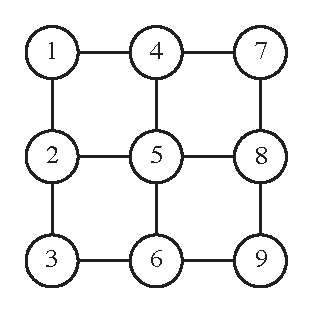
\includegraphics[width=.3\textwidth]{figures/epbp/grid33}
	\hspace*{1cm}
	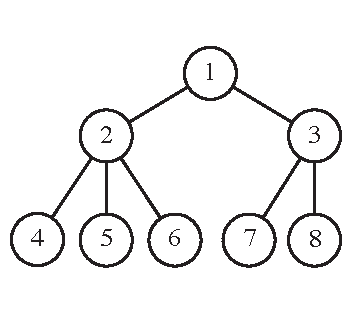
\includegraphics[width=.3\textwidth]{figures/epbp/tree8}
%\vspace*{-.5cm}
	\caption{\label{fig:grids}Illustration of the grid (left) and tree (right) graphs used in the experiments.}
\end{figure}

PBP as presented in \citet{ihler09} is implemented using the same parameters than those in an implementation code provided by the authors: the proposal on each node is the last estimated belief and sampled with a 20-step MCMC chain, the Metropolis Hastings proposal is a normal distribution. For EPBP, the approximation of the messages are Gaussians. The ground truth is approximated by running LBP on a deterministic equally spaced mesh with 200 points. All simulations were run with Julia on a Mac with 2.5 GHz Intel Core i5 processor, our code is available online.\footnote{\url{https://github.com/tlienart/EPBP}.} All the experiments were run multiple times as shown on the figures to account for the inherent stochasticity of the methods. The mean trends are also drawn.
%%%%%%%%%%%%%%%%%%%%%%%%%%%
%\subsubsection{Results of the grid and tree experiments}

Figure \ref{figCompGrid} compares the performances of both methods. The error is computed as the mean $L^{1}$ error over all nodes between the estimated beliefs and the ground truth. One can observe that not only does PBP perform worse than EPBP but also that the error plateaus with increasing number of samples. This is because the sampling within PBP is done approximately and hence the consistency of the estimators is lost. Note that for EPBP, one observes the expected $1/\sqrt{N}$ convergence of particle methods discussed in \citet{ihler09}.

\begin{figure}[!h]
\center
%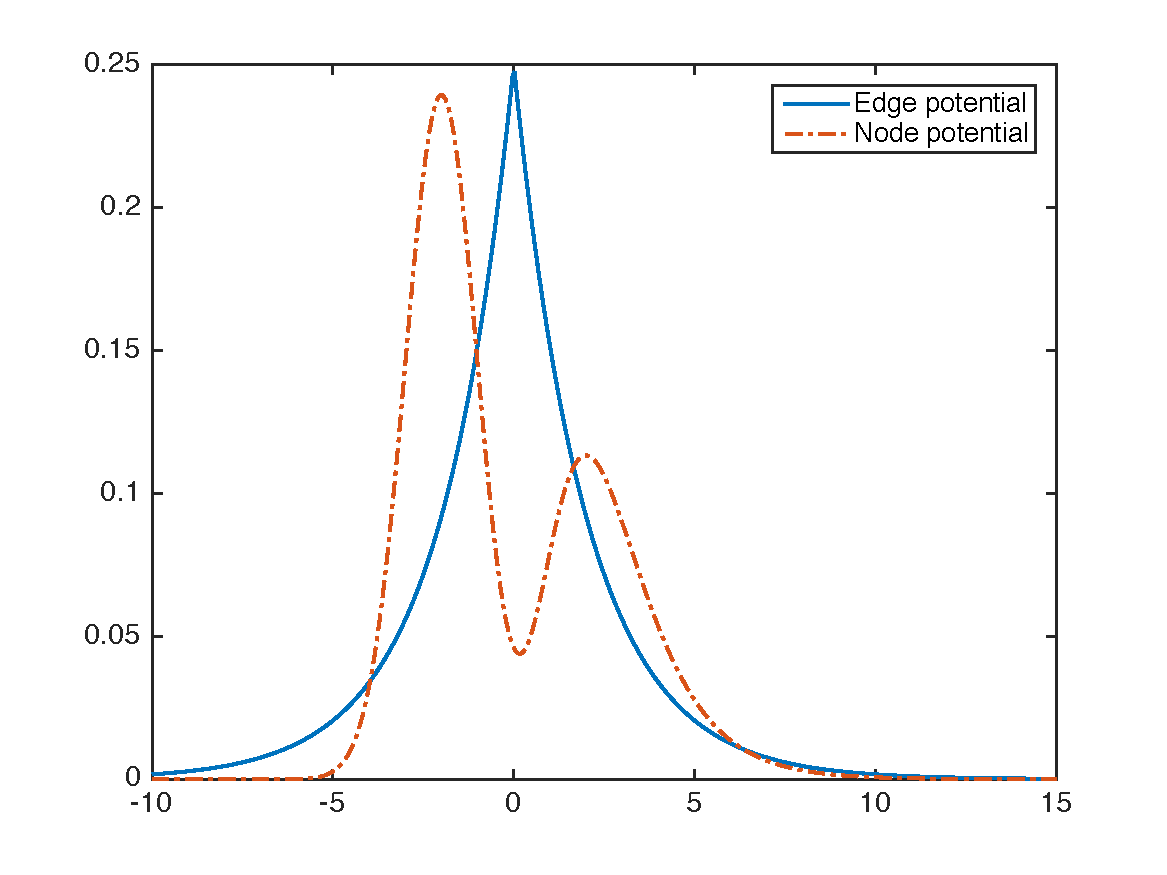
\includegraphics[scale=.25]{figs/node_edge_pot}
%\hspace*{-.6cm}
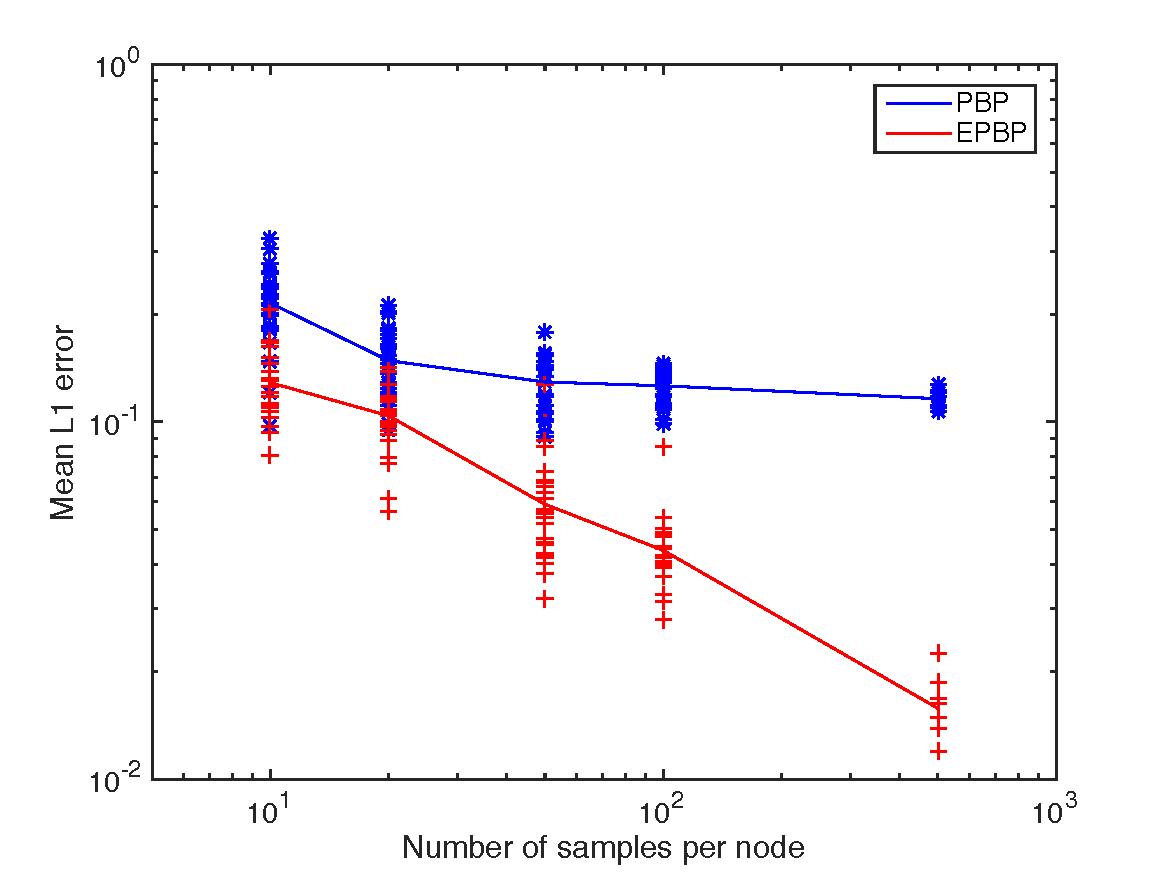
\includegraphics[width=.6\textwidth]{figures/epbp/errComparison}
%\hspace*{-.5cm}
%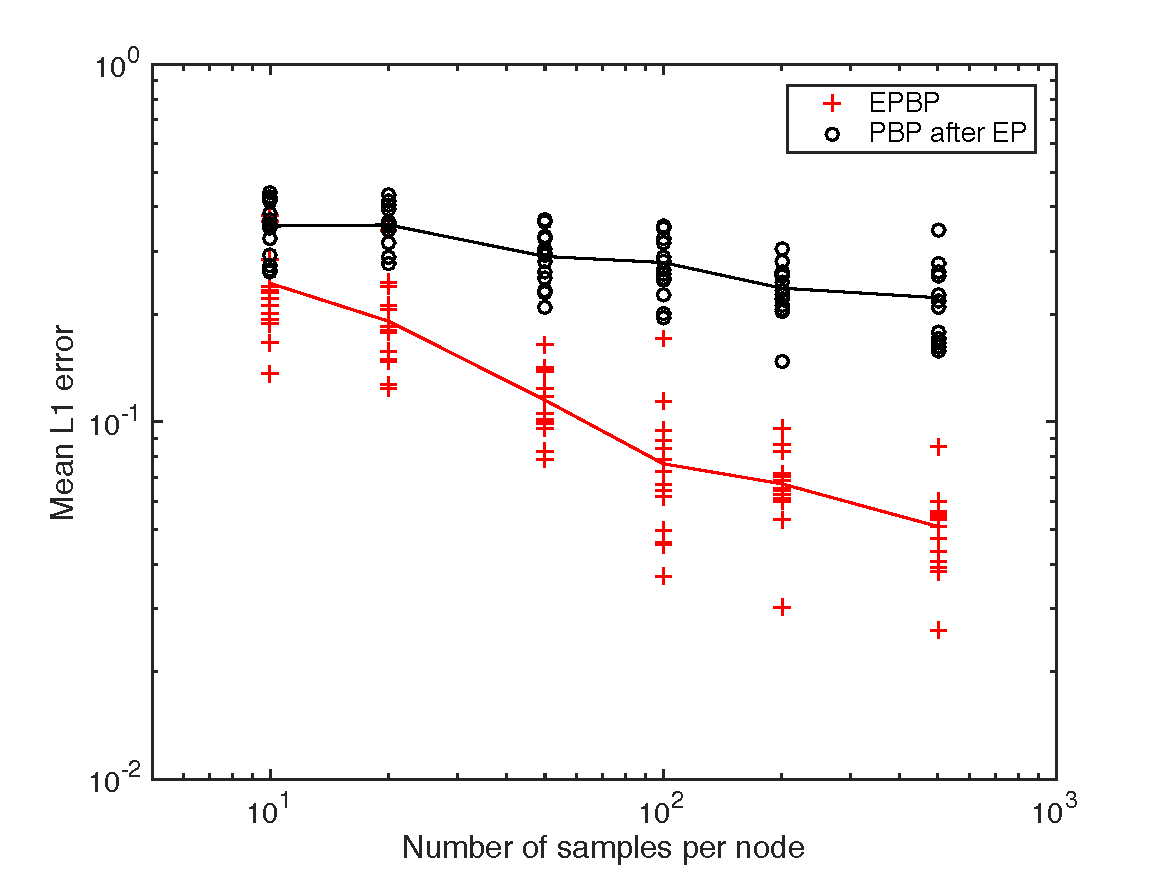
\includegraphics[scale=.35]{figures/epbp/errComparisonEP}
%\vspace*{-.3cm}
\caption{\label{figCompGrid}Comparison of the mean $L^{1}$ error for PBP and EPBP for the $3\times 3$ grid example. EPBP is more accurate for the same number of samples.} %(right) Comparison of the mean $L^{1}$ error for ``PBP after EP'' and EPBP for the tree example. In both cases, EPBP is more accurate for the same number of samples. }
\end{figure}

Figure \ref{compEstBelGrid} compares the estimator of the beliefs obtained by the two methods for three representative nodes (node $1$, $5$ and $9$ as illustrated in \fig{fig:grids} (left)). The figure also illustrates the last proposals constructed with our approach and one can notice that their supports match closely the support of the true beliefs.

\begin{figure}[!h]
%\vspace*{-.5cm}
\center
	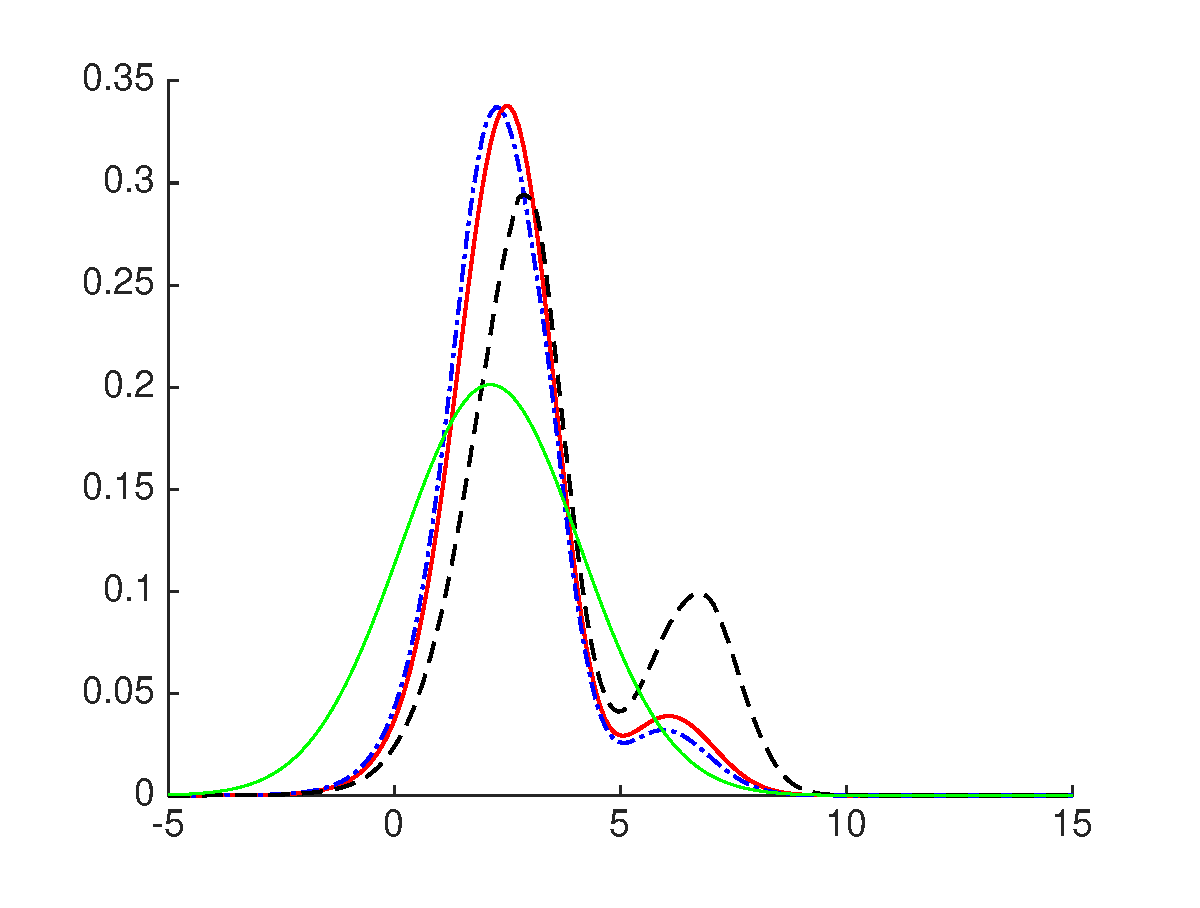
\includegraphics[width=.48\textwidth]{figures/epbp/Gnode1}
	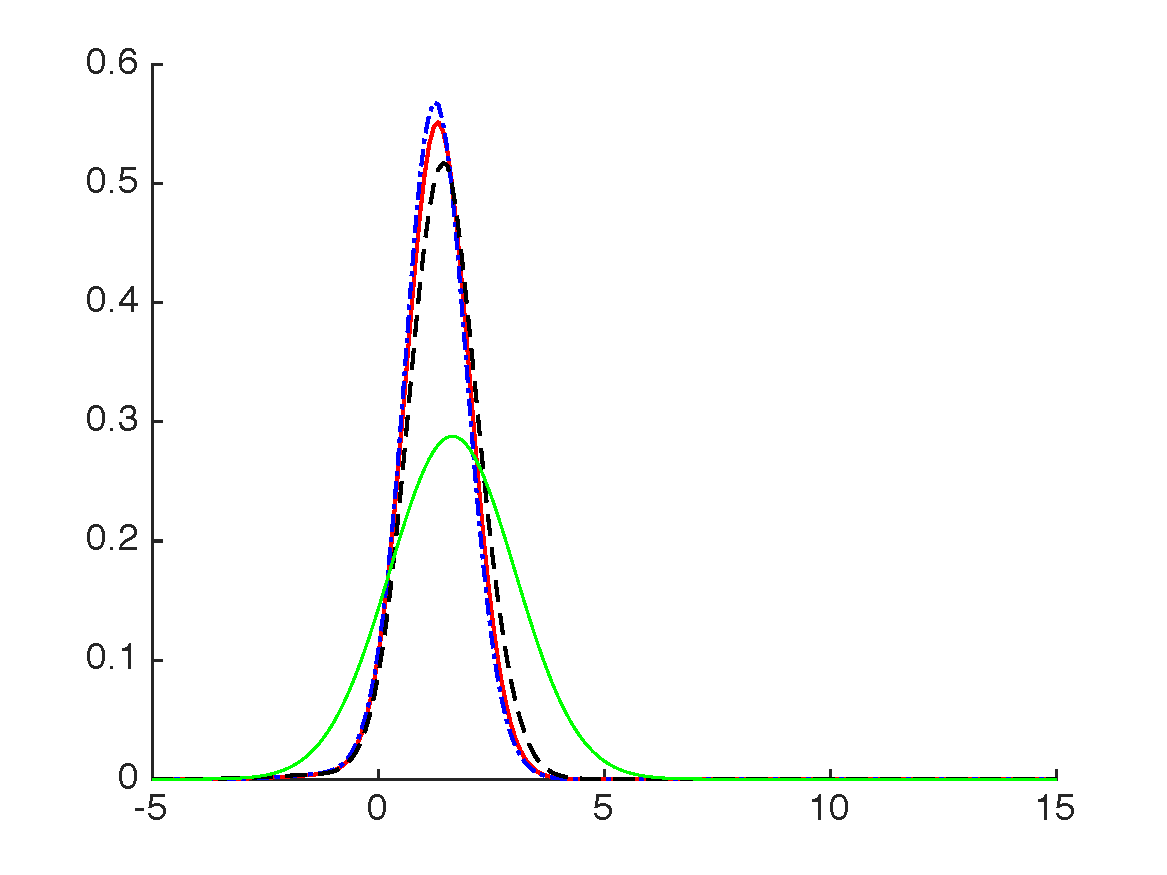
\includegraphics[width=.48\textwidth]{figures/epbp/Gnode5}
	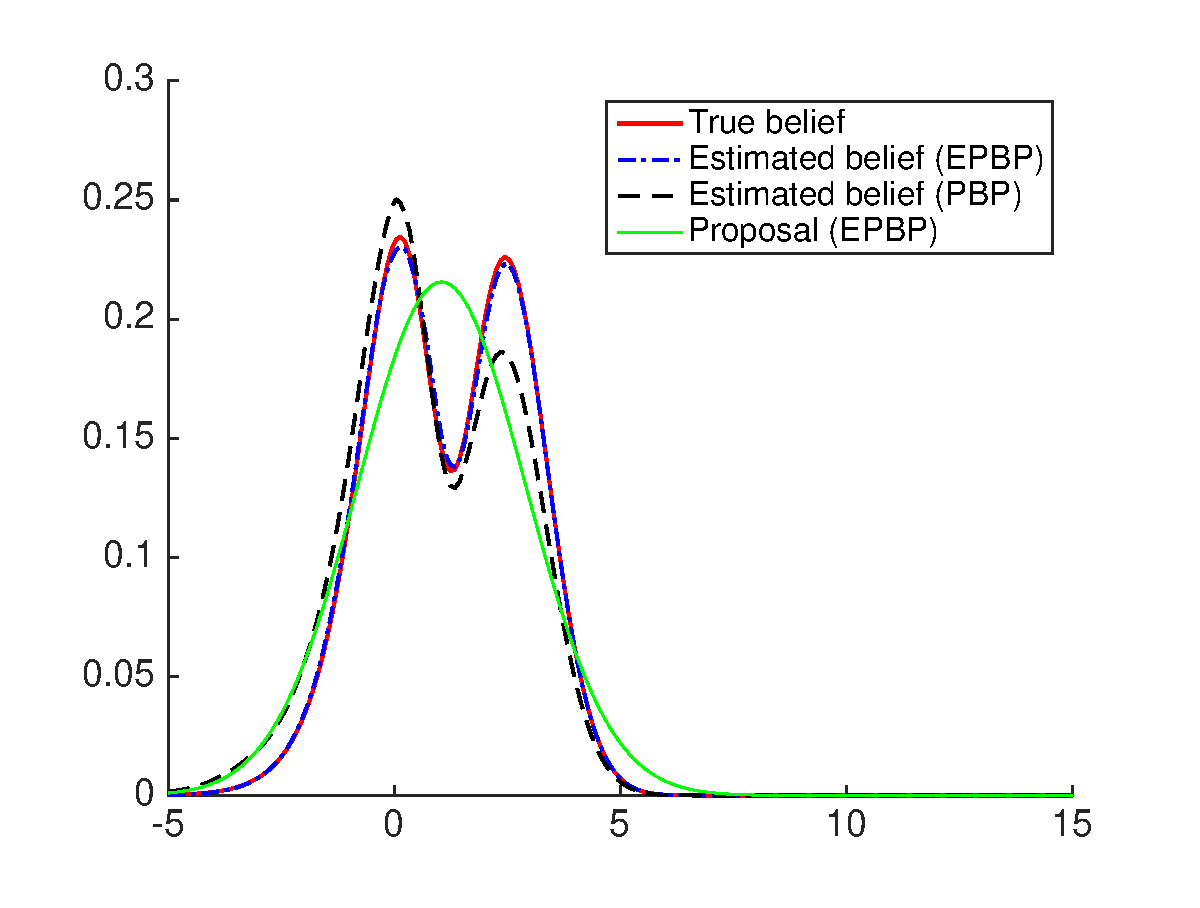
\includegraphics[width=.48\textwidth]{figures/epbp/Gnode9}
%	\vspace*{-.8cm}
%	\hspace*{-.3cm}
%	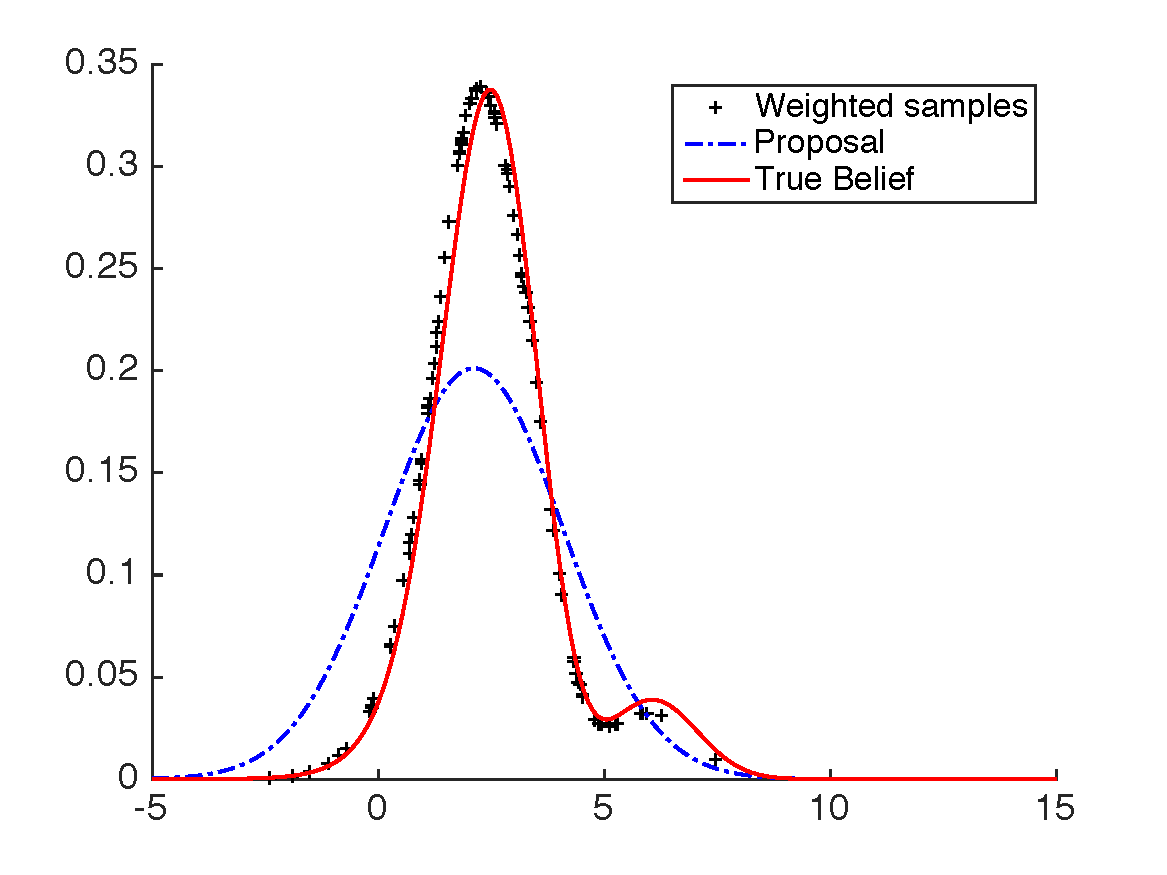
\includegraphics[scale=.25]{figs/node1_epbp}
%	\hspace*{-.5cm}
%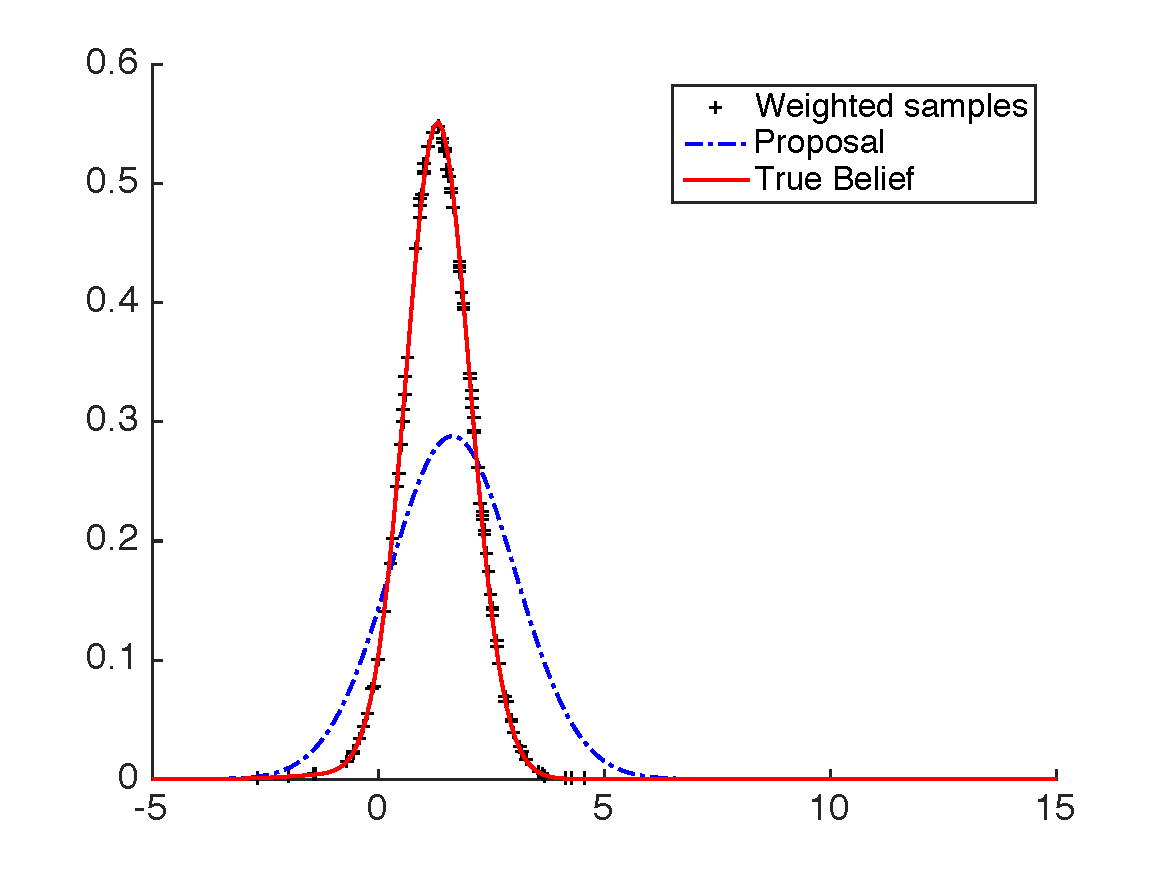
\includegraphics[scale=.25]{figs/node5_epbp}
%	\hspace*{-.5cm}
%	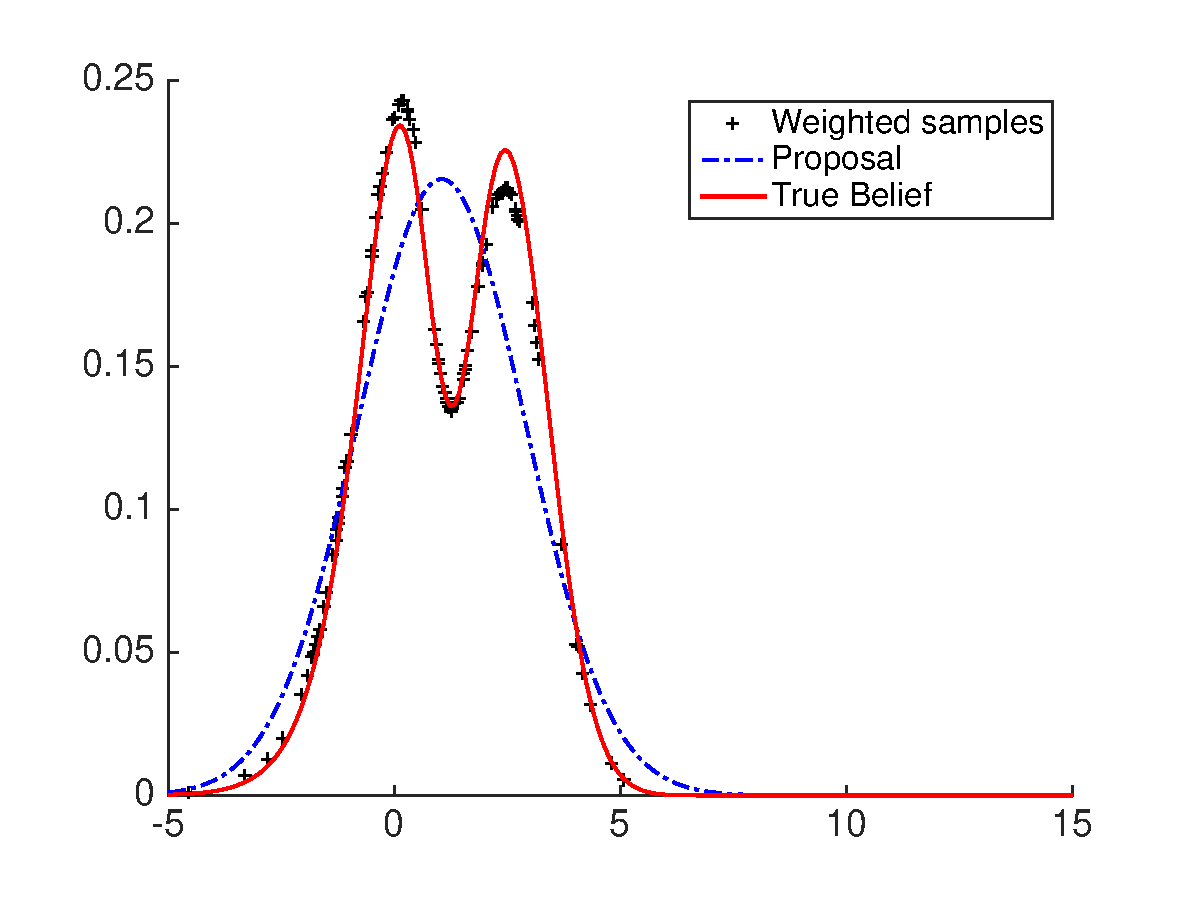
\includegraphics[scale=.25]{figs/node9_epbp}
\caption{\label{compEstBelGrid}Comparison of the beliefs on node $1$, $5$ and $9$ (top left, top right, bottom) as obtained by evaluating LBP on a deterministic mesh (\emph{true belief}), with PBP and with EPBP for the $3\times 3$ grid example. All three plots share the same legend. The proposal used by EPBP in the last step is also illustrated. The results are obtained with $N=100$ samples on each node and $20$ BP iterations. One can observe visually that EPBP outperforms PBP.}
\end{figure}

The speed-up offered by EPBP is very substantial as can be seen in \fig{compConv} (left). Hence, although it would be possible (and sensible) to use more MCMC iterations within PBP to improve its accuracy, it would make the method prohibitively expensive to use compared to EPBP. Figure \ref{compConv} (right) illustrates how the estimated beliefs converge as compared to the true beliefs with increasing number of loopy belief propagation iterations. One can observe that PBP converges more slowly and that the results display more variability which is likely also due to the MCMC runs being too short. %Making them longer is unpractical however as the computational complexity is already higher than that of EPBP.

%
%
%%\newpage
%
%
%
%% THIS IS from THE /DATAMIXNG/ folder

%
\begin{figure}[!h]
\center
%\vspace*{-.5cm}
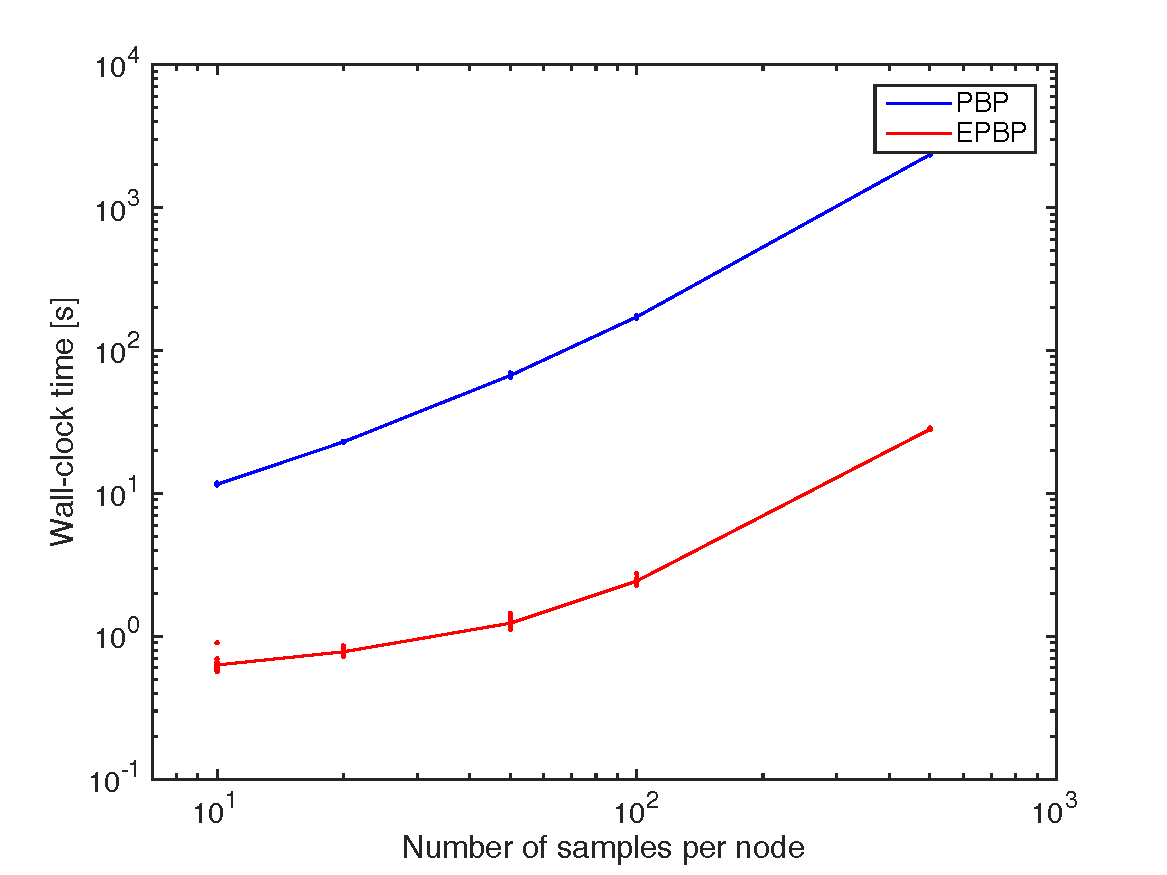
\includegraphics[width=.51\textwidth]{figures/epbp/timeComparison}
\hspace*{-.7cm}
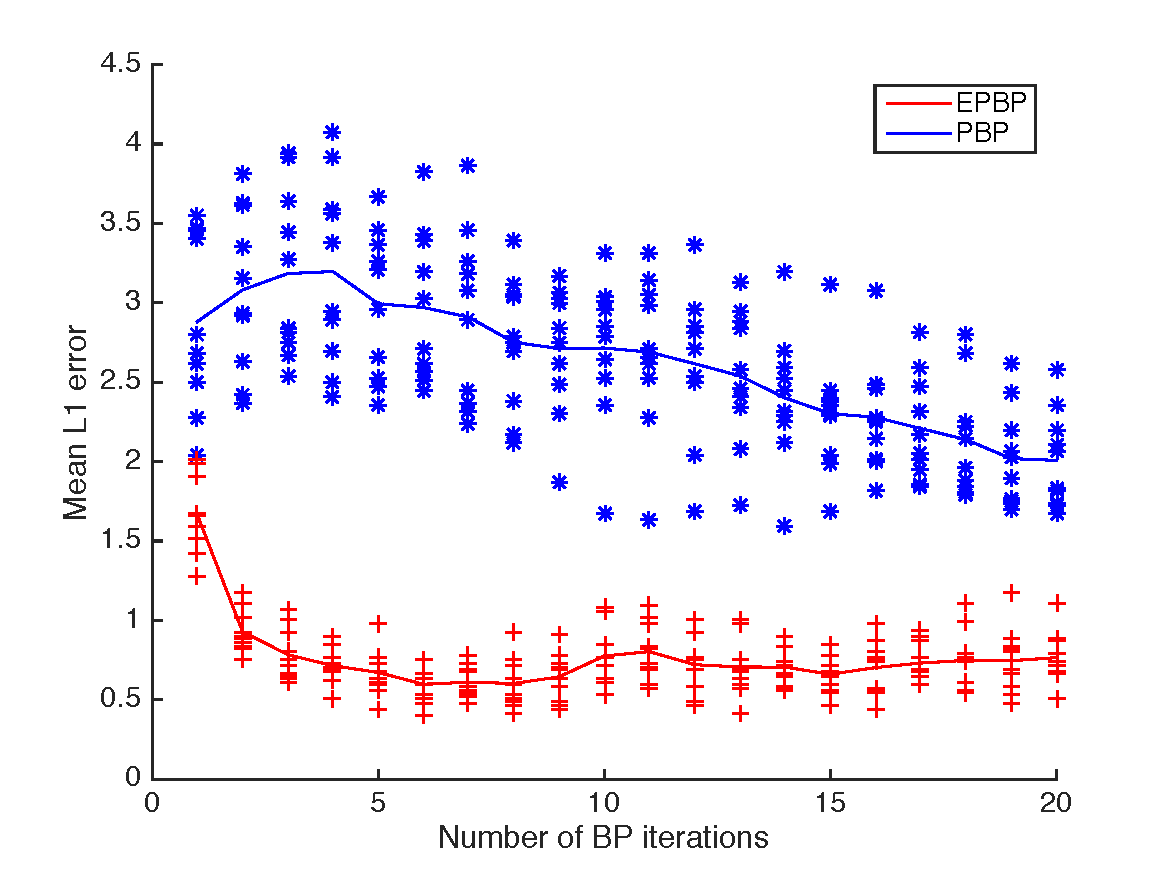
\includegraphics[width=.51\textwidth]{figures/epbp/compBPconv}
%
%\vspace*{-.4cm}
\caption{\label{compConv} (\textbf{left}) Comparison of the wall-clock time needed to perform PBP and EPBP on the $3\times 3$ grid example. (\textbf{right}) Comparison of the convergence in $L^{1}$ error with increasing number of BP iterations for the $3\times 3$ grid when using $N=30$ particles. }%(right) }
\end{figure}
%
%
%\newpage
%
The same experiments were also run on the tree example with similar results.
Additionally, we looked at how ``pure EP'' with normal distributions performs. We also tried using the distributions obtained with EP as proposals for PBP (referred to as ``PBP after EP'' in figures). All those methods underperform compared to EPBP. In particular one can observe in \fig{compPBPaEP} that ``PBP after EP'' converges slower than EPBP with increasing number of samples.
%
%
%
\begin{figure}[!h]
\center
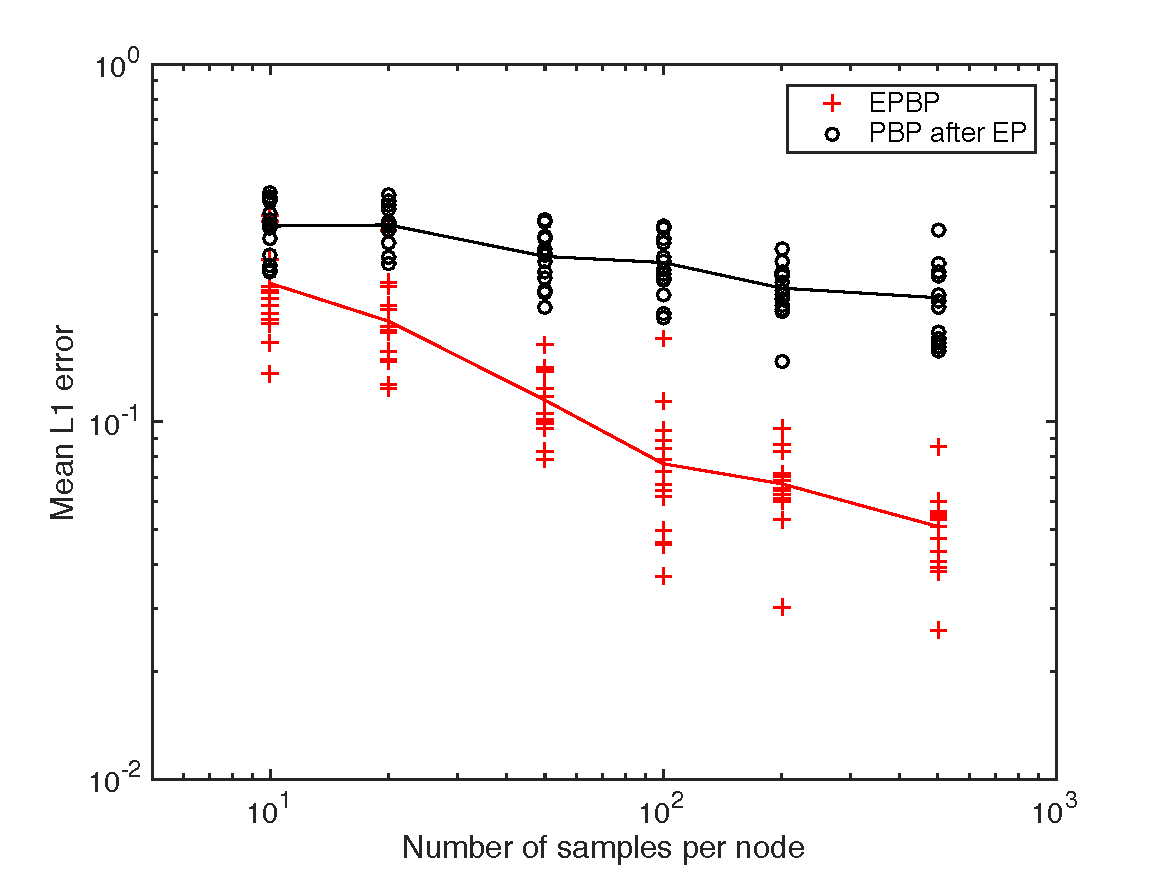
\includegraphics[width=.6\textwidth]{figures/epbp/errComparisonEP}
\caption{\label{compPBPaEP}Comparison of the mean $L^{1}$ error for EPBP and ``PBP after EP'' for the tree example. EPBP is more accurate and converges faster.}
\end{figure}


Figure \ref{compTree} compares the estimator of the beliefs obtained by all the methods on the tree example for three representative nodes (node $1$, $3$ and $8$ as illustrated in \fig{fig:grids} (right)). As for the grid example, the figure illustrates how EPBP better recovers the true beliefs. 


\begin{figure}[!h]
\center
%\vspace*{-.2cm}
%	\hspace*{-.3cm}
	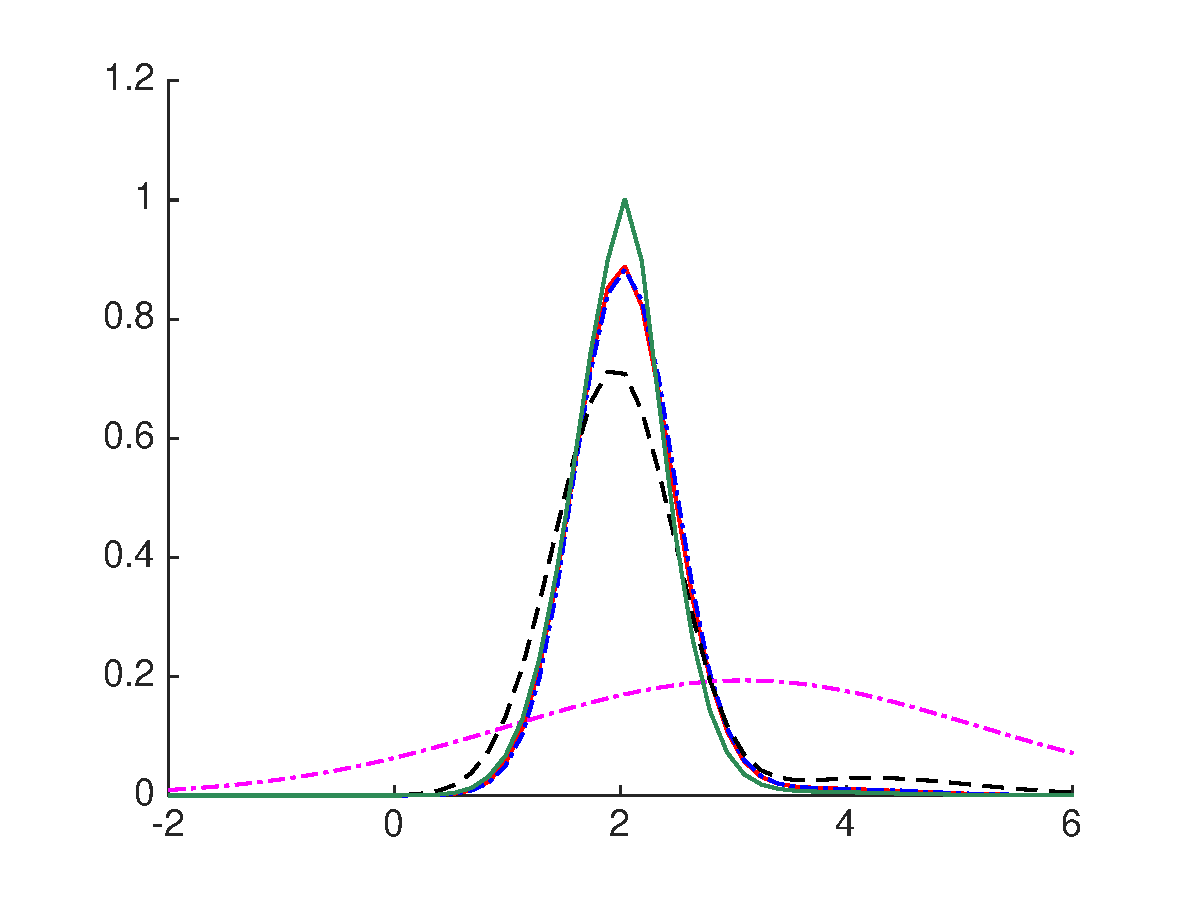
\includegraphics[width=.48\textwidth]{figures/epbp/tree_node1}
%	\hspace*{-.5cm}
	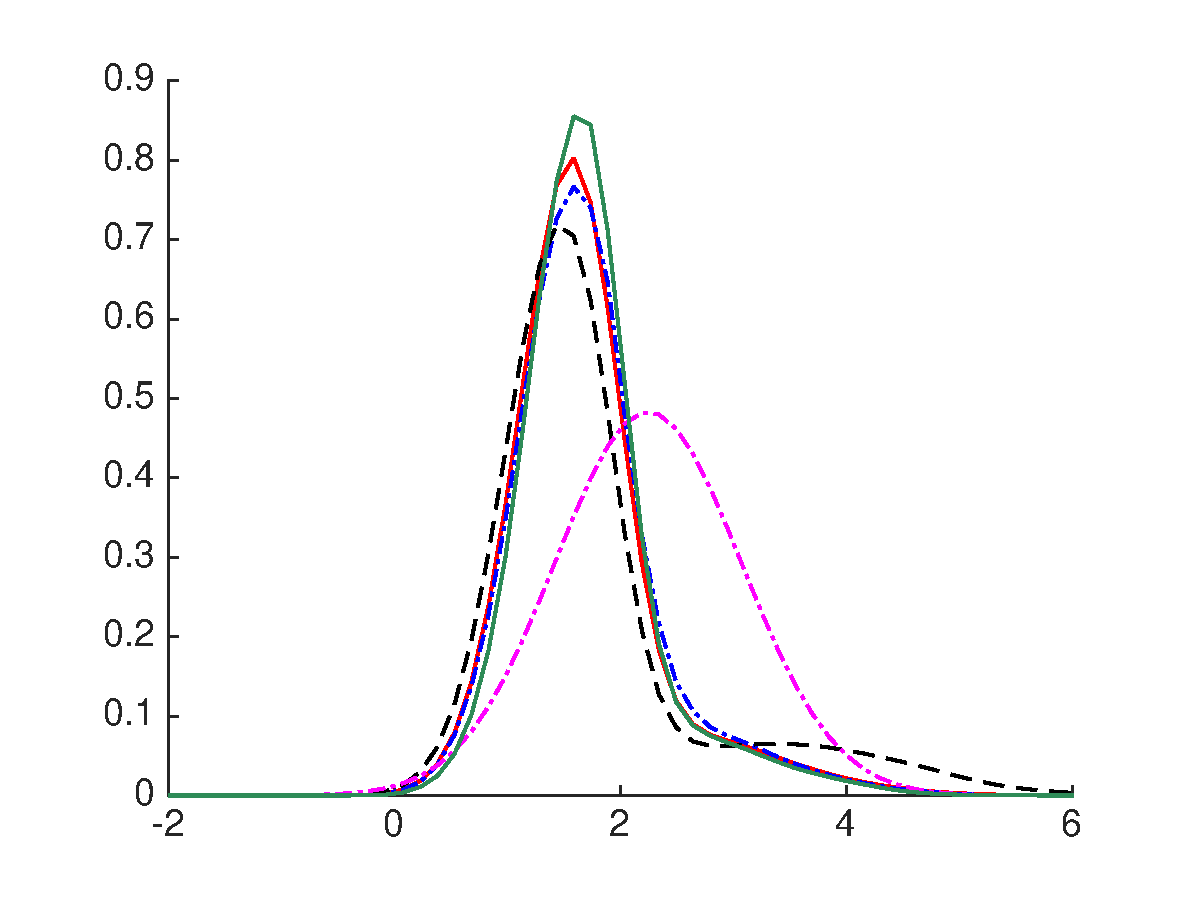
\includegraphics[width=.48\textwidth]{figures/epbp/tree_node3}
%\hspace*{-.5cm}
	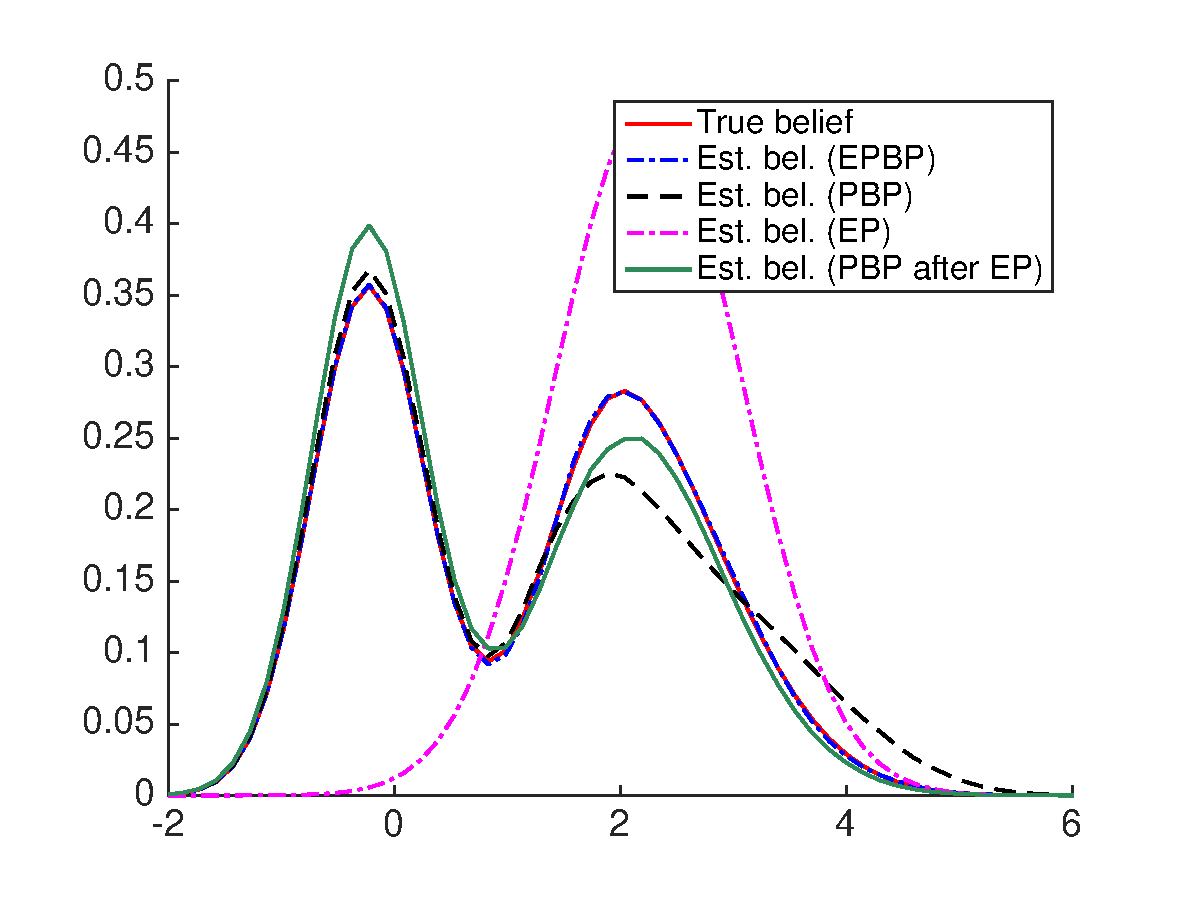
\includegraphics[width=.48\textwidth]{figures/epbp/tree_node8}

	\caption{\label{compTree}Comparison of the beliefs on node $1$, $3$ and $8$ (top left, top right, bottom) as obtained by evaluating LBP on a deterministic mesh, using EPBP, PBP, EP and PBP using the results of EP as proposals. All three plots share the same legend. This is for the tree example with $N=100$ samples on each node and $20$ LBP iterations. Again, one can observe that EPBP outperforms the other methods. }
\end{figure}

\subsection{Sub-quadratic implementation and denoising application}
As outlined at point \ref{sec:EPBP-compcompl}, the inherent quadratic complexity of the EPBP algorithm can be reduced to $\mathcal O(MN)$ where $M$ is the number of mixture components effectively considered to represent the messages. We also consider the maximum likelihood-based projection mechanism as discussed in section \ref{point:epbp-proj} for the two experiments.

We apply this method to the $3\times 3$ grid example in the case where $M=\mathcal O(\log(N))$: for $N=\{10,20,50,100,200,500\}$, we pick $M=\{5, 6,8,10,11,13\}$. The results are illustrated in \fig{figCompNLOGN} where one can see that the $N\log N$ implementation compares very well to the original quadratic implementation at a much reduced cost. 


\begin{figure}[!h]
%\vspace*{-.7cm}
\center
%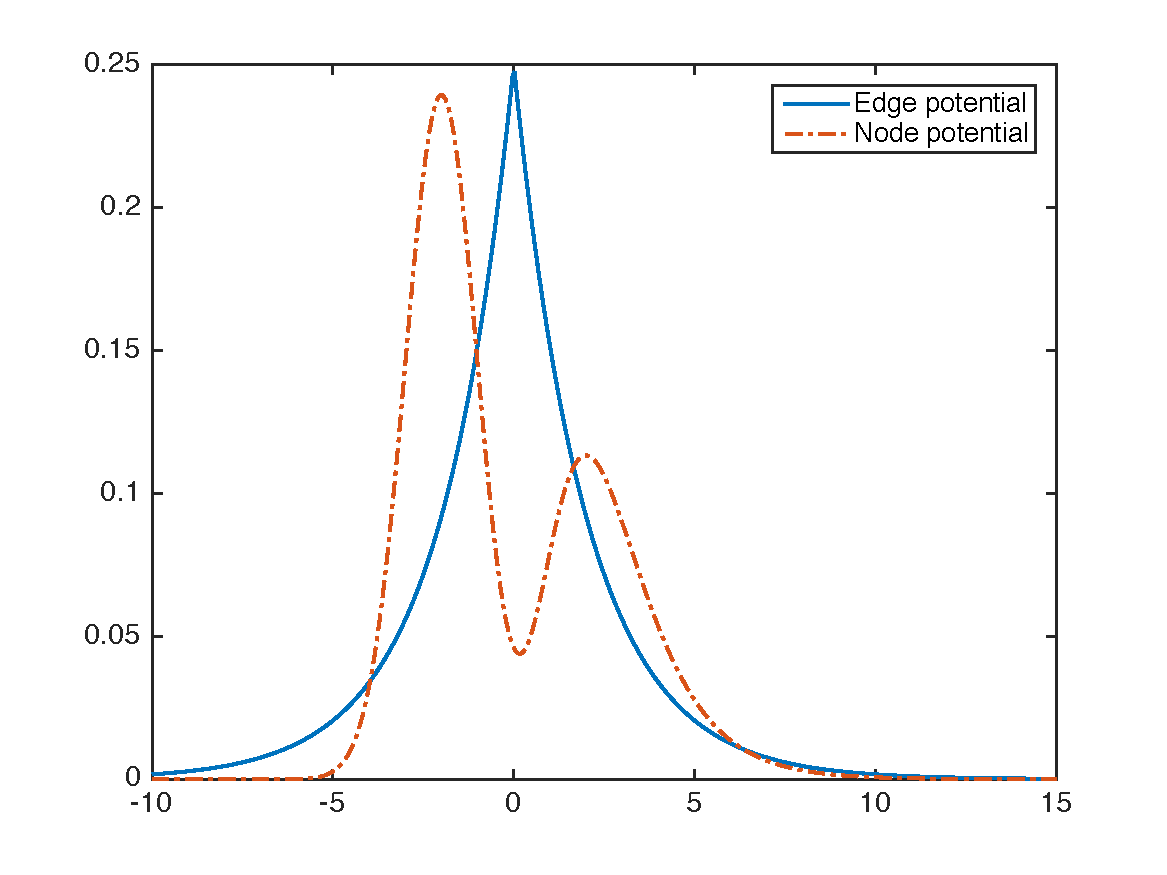
\includegraphics[scale=.25]{figs/node_edge_pot}
%\hspace*{-.6cm}
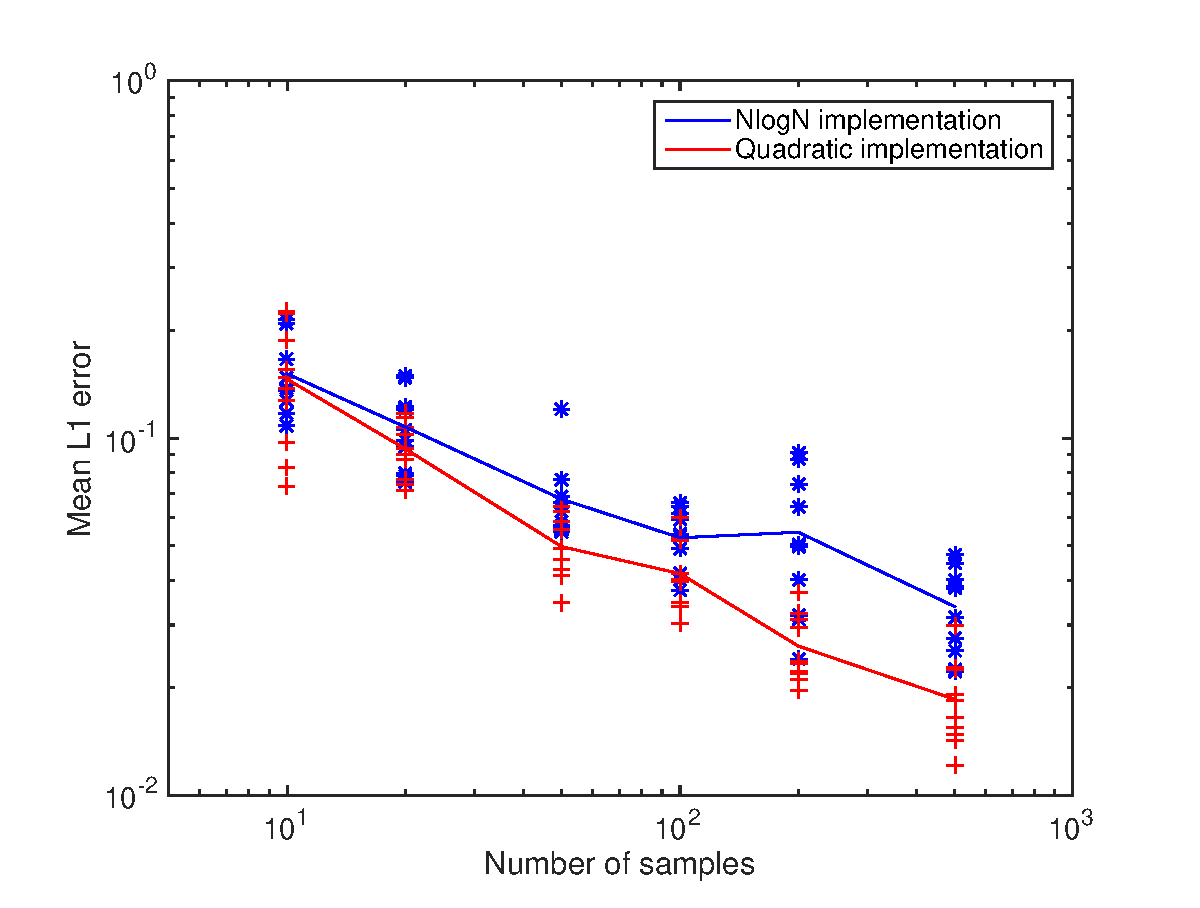
\includegraphics[width=.51\textwidth]{figures/epbp/errCompNLOGN}
\hspace*{-.7cm}
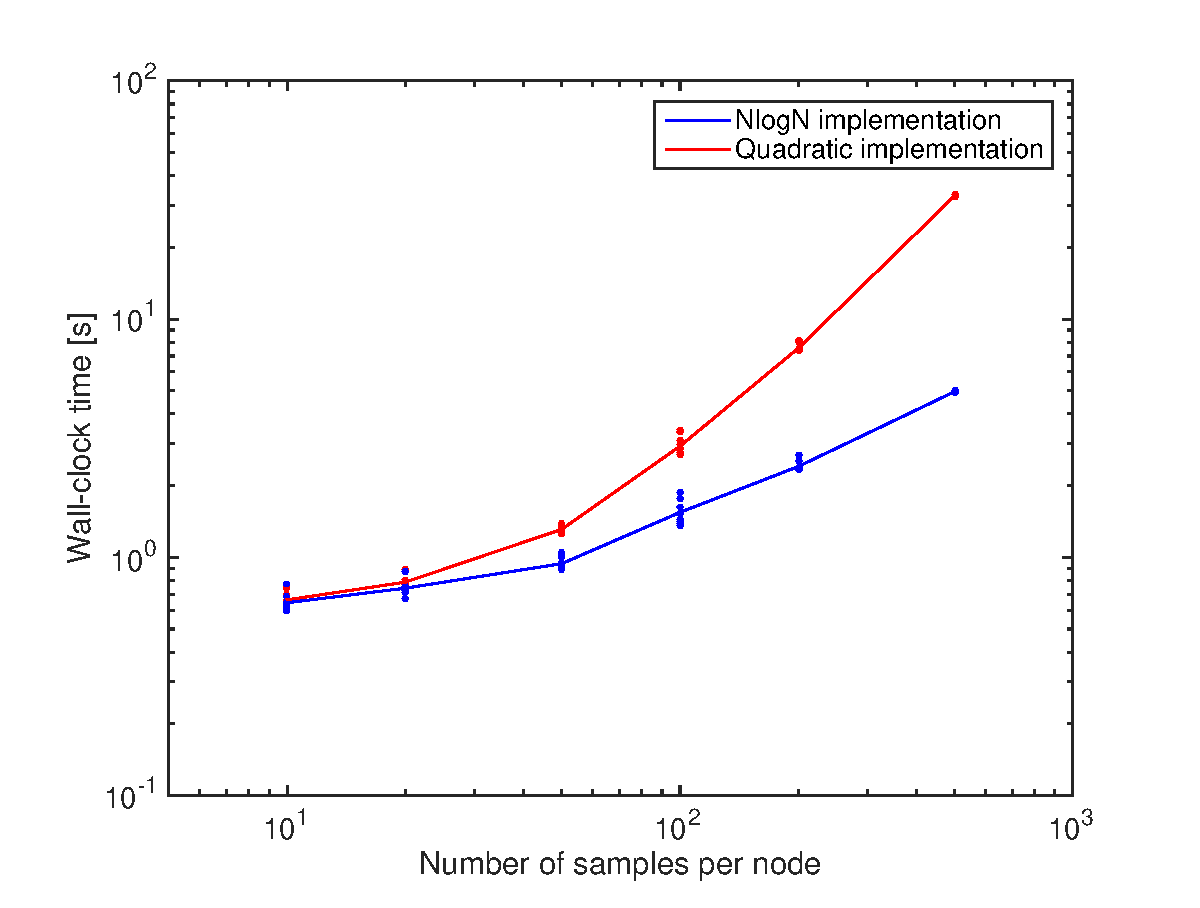
\includegraphics[width=.51\textwidth]{figures/epbp/timeCompNLOGN}
%\vspace*{-.4cm}
\caption{\label{figCompNLOGN}Comparison of the quadratic and $\mathcal O(N log N )$ implementations. (\textbf{left}) Comparison of the mean L1 error, (\textbf{right}) comparison of the wall-clock time. The sub-quadratic implementation performs almost as well as the original implementation and offers a significant speedup.}
\end{figure}


We apply the same sub-quadratic method on a simple probabilistic model for an image denoising problem. The aim of this example is to show that the method can be applied to larger graphs and still provide good results. The model underlined is chosen to showcase the flexibility and applicability of our method in particular when the edge-potential is non-integrable. It is not claimed to be an optimal approach to image denoising.\footnote{In this case in particular, an optimisation-based method such as that of \citet{rudin92} is very likely to yield better results and much faster.}

The node and edge potentials are defined as follows:
\eqa{	
	\left\{
		\begin{array}{lcl}
			\psi_{u}(x_{u}) &=& \mathcal N(x_{u}-y_{u};0,0.1)\\
			\psi_{uv}(x_{u},x_{v}) &=& \mathcal L^{\lambda}(x_{u}-x_{v};0,0.03)
		\end{array}
	\right.,\label{modelIMG}
}
where $\mathcal L^{\lambda}(x;\mu,\beta)=\mathcal L(x;\mu,\beta)$ if $|x|\le \lambda$ and $\mathcal L(\lambda;\mu,\beta)$ otherwise. In this example we set $\lambda=0.2$. The value assigned to each pixel of the reconstruction is the estimated mean of the belief obtained over the corresponding node (figure \ref{figIMG}). The image has size $50\times 50$ (therefore corresponding to a grid graph of 2500 nodes) and the simulation was run with $N=30$ particles per nodes, $M=5$ and $10$ BP iterations taking under 2 minutes to complete with the setup described earlier. 
We compare it with the result obtained with EP on the same model. 
Running PBP or any other quadratic method on this example is prohibitively expensive due to the size of the underlying graph.

\begin{figure}[!h]
\center
%\hspace*{-2cm}
%\vspace*{-.4cm}
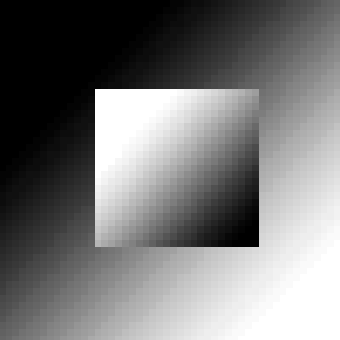
\includegraphics[scale=.28]{figures/epbp/denoisingExpleORIG}
\hspace*{.3cm}
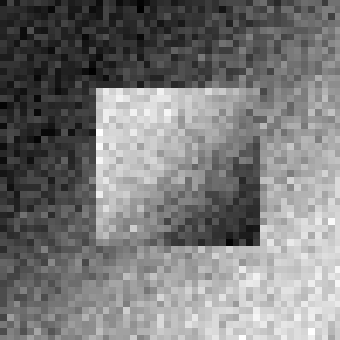
\includegraphics[scale=.28]{figures/epbp/denoisingExpleINPUT}
\hspace*{.3cm}
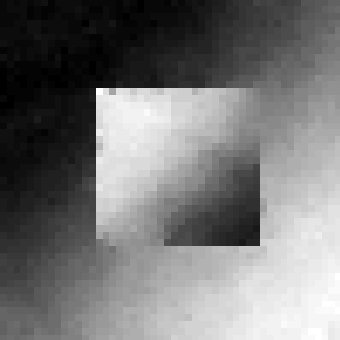
\includegraphics[scale=.28]{figures/epbp/denoisingExpleRECO}
\hspace*{.3cm}
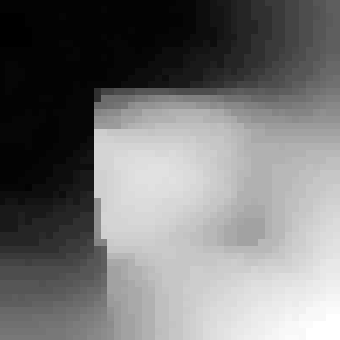
\includegraphics[scale=.28]{figures/epbp/denoisingEP2}
%\hspace*{-1.5cm}
%\vspace*{-.3cm}
\caption{\label{figIMG} From left to right: comparison of the original (first), noisy (second) and recovered image using the sub-quadratic implementation of EPBP (third) and with pure EP (fourth). % with $N=30$ samples per nodes and $10$ BP iterations with the model \eqref{modelIMG}.
}
\end{figure}

% >>>>>>>>>>>>>>>>>>>>>>>>>>>>>>
% >>>>>>>>>>>>>>>>>>>>>>>>>>>>>>
% >>>>>>>>>>>>>>>>>>>>>>>>>>>>>>
% >>>>>>>>>>>>>>>>>>>>>>>>>>>>>>

%%%%%%%%%%
\section{Discussion}

In this chapter, we presented an original way to design adaptively efficient and easy-to-sample-from proposals for a particle implementation of the LBP algorithm. The construction of proposals is done in the Expectation Propagation framework.

We have demonstrated empirically that the resulting algorithm is significantly faster and more accurate than an implementation of the PBP algorithm using the estimated beliefs as proposals and sampling from them using MCMC as proposed in \cite{ihler09}. 
It is also more accurate than using plain EP due to the nonparametric nature of the messages and offers consistent estimators of the LBP messages. 

A sub-quadratic version of the method was also outlined and shown to perform almost as well as the original method on mildly multi-modal models, it was also applied successfully in a simple image denoising example illustrating that the method can be applied on graphical models with thousands of nodes at a reasonable computational cost.

We believe that our method could be applied successfully to a wide range of applications requiring good approximation of the marginals of continuous MRF such as smoothing for Hidden Markov Models \cite{briers10}, tracking or computer vision \cite{sudderth04,felzenszwalb04}. 

%\subsubsection*{Possible paths for future work}

As discussed in point \label{point:epbp-proj}, other projection mechanisms than the KL projection can be considered. We could also look at other discrepancy measure than the KL such as $\alpha$-divergences. This latter choice would suggest considering the power-EP framework \citep{minka04} and could be justified if we seek to build representations of the messages with specific properties. It is unclear to us however how the choice of power in power-EP affects the quality of the proposals representing the node beliefs nor how it would affect the performances of the algorithm.

%To conclude, note that the NBP algorithm of \citet{sudderth03} may in fact be sufficient for a large number of practical applications where MRF does verify the integrability conditions \eqref{conditions NBP} and if the beliefs are not expected to be highly multimodal or non-Gaussian. In a way the NBP algorithm can be compared with the Kalman filter and smoother for a HMM and related techniques: as a first go-to method which may, in fact, lead to satisfactory results. In situations where the NBP algorithm fails or is not applicable, the EPBP algorithm could prove to be a more sensible choice than the PBP algorithm.


